\documentclass{article}
\usepackage{amsmath,amssymb,setspace,verbatim,graphicx,enumerate,enumitem}
\usepackage[top=1in,bottom=1in,left=1in,right=1in,head=0.5in,foot=0.5in]{geometry}
\usepackage{caption}
\usepackage{mathtools}
% \usepackage{subcaption}
% \usepackage{subfig}
% \usepackage{subfloat}
% \usepackage{tabularx}
\usepackage{mdframed}
\usepackage{amsthm}

\newtheorem*{theorem}{Theorem}
\newtheorem*{definition}{Definition}

\newenvironment{Rcode}% environment name 
{%begin code
    \begin{mdframed}
    \#R code
    \begin{small}
}
{%end code
    \end{small}
    \end{mdframed}
}

\newenvironment{console}% environment name 
{%begin code
    \begin{mdframed}
    \#Console
    \begin{small}
}
{%end code
    \end{small}
    \end{mdframed}
}

\begin{document}
\title{STDA Final Project: \\ More general covariance structures for spatio-temporal models}
\author{Seokjun Choi}
\date{June 19, 2020}
\maketitle

\textbf{Note:}
You can get tex file of this report at my github page: Visit https://github.com/letsjdosth/SpaTempoDA
You may use it to write a review report.

\section{Introduction}

Spatio-temporal models are different comparing to ordinary model, and the biggest difference is that
the models have some parts that catch a correlation structure between data points.
And imposing this structure, the covariance function plays central role.
So, in this report, I will explain some methods to get or make a valid covariance function for space-time data analysis model.
I will start from the simplistic case which assumes isotropy, separable and symmetry,
and will remove each one, with introducing new concepts and more general covariance structure.
\begin{definition}
    Assume second-stationary spatial process and let C(h) be the covariance function of the process, where $h\in\mathbb R^n$ is space-lag.
    $C$ is isotopic if $C(h)=C(||h||)$, where $||\cdot||$ is norm of the domain.
    $C$ is symmetric if $C(h)=C(-h)$.
\end{definition}
\begin{definition}
    Assume second-stationary spatio-temporal process and let C(h,u) be the covariance function of the process, where $h\in\mathbb R^n$ is space-lag and $u\in\mathbb R$ is time-lag.
    C is separable if $C(h,u)=C_1(h)C_2(u)$ for some $C_1$ and $C_2$.
\end{definition}

\section{Isotopy-related issues}
\subsection{For only spatial (no temporal part) data}
Assume that we work with second-order stationary random field.
First, here is classical method to construct isotropic covariance without proof.
\begin{theorem}{(Schoenberg, 1938)}
    Isotropic function
    \[C(h)=\phi(||h||^2),h\in\mathbb R^d\]
    is a spatial covariance function for all dimension $d$ if and only if $\phi(t)$ has a form $\int e^{-rt}dF(r)$.
\end{theorem}
More detailed version is here.
\begin{theorem}{(Yalgom, 1987)}
    Isotropic continuous covariance of $\mathbb R^d, d\geq 2$ is specified by
    \[c(h)=2^{(m-2)/2} \Gamma(m/2) \int_0^\infty \frac{J_{(m-2)/2}(\omega h)}{(\omega h)^{(m-2)/2}}dF(\omega), h\geq 0\]
    where $h$ is norm of space-lag vector and $J_(.)$ is the Bessel function of order $(.)$.
\end{theorem}
This theorem specifies the structure totally. So, the story related to constructing isotopic covariance for spatial data is finished.



\subsection{Expand the notion of isotopy to spatio-temporal data}
It is obviously unreasonable to deal time axis and space axises as entirely same things because their measurement unit and permitted domain are totally different.
So, different definitions for covariance of space-time data are proposed. 

\begin{definition}
    Let $C(h,u)$ be a space-time covariance function where $h$ be space lag and $u$ be time lag.
    \begin{itemize}
        \item Gneiting et al.(2007)'s spatial isometry : $C(h,u)=C(||h||,||u||)$
        \item Stein(2005)'s spatial isometry : $C(h,0)=C(||h||,0)$
    \end{itemize}    
\end{definition}
Both two case are said 'partial isometry'.
Note that Stein's one is weaker restriction than Gneiting. But Stein claims that his one is the only one that is physically justified.

Construction the covariance structure are easy: just use the form which $h,u$ affect the covariance value through $||h||, ||u||$
as long as keeping positive-definiteness.


\subsection{anisotropic covariances}
Many researchers try to construct covariance function outside isotopy. Here are developed concepts.
All things assumes that second-order stationary random field. Let $h$ be lag-vector and $C_0,C_1,C_2$ be some covariance functions.
\begin{itemize}
    \item (geometric anisotropic covariance) $C(h)=C_0(||LH||)$ where $L:=RD$, $D$ is diagonal matrix for scaling, $R$ is rotation matrix.
    \item (zonal anisotropic covariance) $C(h)=C_1(h_1)+C_2(h_2)$ where $h=(h_1,h_2)$.
\end{itemize}
For first case, it allows direction-by-direction non-isotopy. (For detect this, you may use directional variogram. See Allard et al.(2016))
To construct geometric anisotropic covariance, you can just multiply the isotropic covariance to anisotropic covariance function.
Many things are constructed by this manner. Note that if you multiply two anisotropic one, nothing is guaranteed. There are both cases to get isotropic one and not to.
See $C_1(h_1,h_2)=e^{-a_1 h_1^2-a_2 h_2^2}$ and $C_2(h_1,h_2)=a_1' h_1^2-a_2' h_2^2$, where $a_1\neq a_1', a_2 \neq a_2'$, $a_1,a_2,a_1',a_2'>0$.
Although $C_1$ and $C_2$ are anisotropic, if $a_1+a_1'=a_2+a_2'$, the product $C_1(h_1,h_2)C_2(h_1,h_2)$ become isotropic.

For second case, it factors to two subspace (in fact, you can split it more) and give covariance structure for each one,
but this idea has some fault: for intermediate direction of two factored space, this structure is fitted poorly.
Also, covariance matrix using the structure is not strictly positive definite so that when you try to krigging,
you may face problem to invert the augmented covariance matrix. So, avoid it if possible.

For more specific example of covariance function, see Porcu et al.(2006).


\section{Separability-related issues}
\subsection{Motivation to non-separable covariance function}
Return to the separable and isotropic covariance case as starting point of this section.
\begin{theorem}
    Let $C$ be continuous covariance function on $\mathbb R^d$ and suppose that the partial derivatives exist on $R^d$.
    Then, $C$ is separable and isotropic, i.e. for $h=(h_1,\dots h_k) \in \mathbb R^{i_1} \times \dots \times \mathbb R^{i_k}=\mathbb R^d$
    \[C(h)=\prod_{j=1}^{k}C_j(h_j)\]
    if and only if $C$ is a Gaussian covariance function, i.e.
    \[C(h)=C(||h||)=e^{-k(h_1^2+\dots+h_d^2)}, k>0\]
    with Euclidean norm.
\end{theorem}
The proof depends on the Maxwell's theorem in probability theory and statistical physics. So I skip the proof.
But idea is here: only rotationally invariant probability distribution on $\mathbb R^d$ that have independent component are multivariate normal distribution with expected value $0$ and variance $\sigma I_d, \sigma>0$.
(Feller, 1966)

The above class is too narrow to fit diversely-correlated data. So, I explore more general structure beyond the isotopic-separable condition.
Unfortunately(maybe fortunately to you), however, central results related to non-separable covariances are introduced in Park's lecture,
so in this section, I introduce more detail process to draw them.


\subsection{Brief review to Fourier analysis}
This subsection is preliminary.
I will use below notations: 
for $f\in L^1$ or $L^2$, $x\in\mathbb R^d$ and $\xi\in\mathbb R^d$, the Fourier transform of $f$ on $\mathbb R^d$ is
\[(f)\hat{ } = \hat{f}(\xi)=\int_{\mathbb R^d}e^{-2\pi i x\cdot \xi}f(x)dx\]
and the inversion formula is
\[(\hat{f})\check{ } = \check{\hat{f}}(x)= \int_{\mathbb R^d} e^{2\pi i x\cdot \xi} \hat{f}(\xi) d\xi\]

It is important to know that above two operation are well defined only on $L^1$ or $L^2$ of $\mathbb R^d$. 
(It is actually false statement because we can expand to upper-half complex plain or to another p using $L^p$-interpolation, but I'll skip it.)
To get the $L^1$ boundedness, transform is followed by the dominated convergence theorem,
and inversion is by direct estimation of difference of $L1$ norm.
To get the $L^2$ boundedness, using the fact that the Schwartz class is dense in $L^2$,
define the notions of transform and inversion as limit of them of Schwartz class's.

Fortunately, we will work only with probability measure, finite on whole space, so in this case, $L^2 \subset L^1$.
So, to check if our situation is valid or not to use Fourier analysis, we just need to know the function $f$ is whether integrable or not.

Also note that because convention for denoting the Fourier transform and inversion in mathematics and statistics are different
for minus sign on exponent part (for example, you may learn in mathematical statistics, the characteristic function,
the Fourier transform of density, as $E(e^{itX})$, no minus there! and if we select{ this notation,
we should add minus sign to the exponent of inversion formula.), but essentially they are same (by applying change of variable).
But, if you are not familiar with both convention, you would be confused easily when I mix them.
So in here, I choose to follow of mathematics from here to end of this report.

Here are some properties of Fourier transform.

\((\hat{f})\check{ } = f\) (so-called, transform and inversion are one-to-one operation each other.)
\((f(x+h))\hat{ } = \hat{f}(\xi) e^{2\pi i \xi \cdot h} \), 
\((f(x)e^{-2\pi i xh})\hat{ } = \hat{f}(\xi+h)\), 
\((f(\delta x))\hat{ } = \delta^{-d}\hat{f}(\delta^{-1}\xi)\) (dilation property), 
\(((\frac{\partial}{\partial x})^\alpha f(x))\hat{ } = (2\pi i\xi)^\alpha \hat{f}(\xi)\), 
\(((-2\pi i x)^\alpha f(x))\hat{ } = (\frac{\partial}{\partial \xi})^\alpha \hat{f}(\xi)\).
All these things are directly showed by the definition so easy to check.
And, because the transform and inversion are integral operator, they are continuous and linear operator.
Also, the transform preserves composed rotation operator, radial property, and $L^2$ norm (when $f \in L^2$, by Plancherel theorem).

\subsection{the Bochner's theorem}
This theorem guarantees the positive-definiteness of a function. (In fact, he is very famous in harmonic analysis, by Bochner-Riesz mean and so on.)

\begin{theorem}{(Bochner,1955)}
Let C(x) be continuous function on $\mathbb R^d$ such that the Fourier transform of C is well-defined.
Then, C is positive definite, in the sense that for all $z_p,z_q \in \mathbb C$ and for any finitely many points $x_1,...,x_N \in \mathbb R^d$,
\[\sum_{p,q=1}^{N} C(x_p-x_q) z_p \bar{z_q} \geq 0\]
if and only if the F in \(C(x)=\int e^{-2\pi i x \cdot y}dF(y)\) is a Borel measure on of real, nonnegative value for any member of its sigma-field,
(in other words, $F$ is a CDF of a random variable).

\end{theorem}
\begin{proof}
    ($\leftarrow$) Since F is always nonnegative and norm of $e^{-2\pi ik}=1$ for all $k$ (just circle in complex plain), 
    \(\int{|\sum_{p=1}^{N} z_p e^{-2\pi i x_p \cdot y} |^2 dF(y)} \geq 0 \). Change the variable $x_p$ to $x_p-x_q$ and use definition of complex norm.
    
    ($\rightarrow$) Observe \(\int\int C(x_p-x_q) z_p \bar{z_q} dx_p dx_q \geq 0\) and bounded, because of finite summation and given conditions.
    plug in $x_p = e^{-\epsilon|\alpha|^2}e^{2\pi i \alpha \cdot y}$ and $x_q = e^{-\epsilon|\beta|^2}e^{2\pi i \beta \cdot y}$ for $\epsilon>0$ and fixed $y$ and
    arbitrary $\alpha, \beta \in \mathbb R^d$. Since $|C(\alpha)| \leq C(0)$ and $|C(\beta)| \leq c(0)$ and \(C(x)=\int e^{-2\pi i x \cdot y}dF(y)\),
    we have \(\int\int e^{-2\epsilon(|\alpha|^2_|\beta|^2)} C(\alpha-\beta) e^{2\pi i \alpha-\beta \cdot y} dv_\alpha dv_\beta \geq 0\)
    Here, apply the change of variable with $\alpha-\beta=\gamma$ and $\alpha-\beta=\delta$, then
    \[\int(\int e^{-\epsilon(|\delta|^2)} dv_\delta) C(\gamma) e^{\epsilon|\gamma|^2} e^{2\pi i \gamma \cdot y} dv_\alpha dv_\gamma \geq 0\]
    Note that the form $e^{-x^2}$ is heat kernel which is 1 if integrate it and is approximation of identity (maybe some dilation is needed but I omit it for simplicity).
    So, combining the fact that the boundedness, above inequality implies $C_\epsilon(\gamma):=e^{-\epsilon |\gamma|^2}C(\gamma)$ belongs to $L^1$ for all $\epsilon>0$.
    Thus when we let $\epsilon \rightarrow 0$, above integral converges to $C(\gamma)$ itself, and it it means that the measure is nonnegative.
    Apply this fact to $C(x)$ and take the measure in the last integral as $F$.
\end{proof}

If we use change of variable $y=-\xi$ to convert the notation of transform-inversion reversely (as above explanation of between two conventions),
we can write as
\[C(x)=\int e^{2\pi i x\cdot \xi} dF\]
Moreover, if $F$ is absolutely continuous (then F is differentiable almost everywhere), we get the pdf $f$ correspond to $F$,
so above result becomes, $c$ is positive definite if and only if
\[C(x) =\int e^{2\pi i x\cdot \xi} f(\xi)d\xi = \check{f}(x)\]

Here is definition.
\begin{definition}
    Let X be random process with covariance function C(x).
    If \(C(x)= \int e^{2\pi i x\cdot \xi} dF(\xi)\), then we call F 'spectral distribution' of the process.
    If the derivative of F, $f(\xi)$, exists, then we call 'spectral density' of the process.
\end{definition}
Note that if $f$ exists, then  $C=\check{f}$, equivalently, $\hat{C}=f$
And I use the term 'space-time side' to call domain of $C$, and 'frequency side' to call the domain of $f$.

\subsection{Crassie-Hwang's approach}
% Prof. Park introduce the non-separable covariance in context of space-time data analysis,

Since we got the Bochner's therorem, Crassie and Hwang(1999)'s work is simplified by a few lines.

Assume that wanted covariance function are of second-order stationary process.
When $h\in \mathbb R^d$ is space-lag and $u\in \mathbb R$ is time-lag of space-time side 
and corresponding frequency side variables $\omega \in \mathbb R^d$,$\tau \in \mathbb R$ respectively,
using the Bochner's theorem with a spectral density $g$, we get
\[C(h,u)= (g)\check{ }_\omega \check{ }_\tau\]
and define $H:=(\omega;u):=(C)\hat{ }_h = (g)\check{ }_\tau$, (then, $H$ is the function on time side $u$ and frequency side $omega$ w.r.t space.)
\[C(h,u)= (H)\check{ }_\omega\]
and they propose the model, which uses $H(\omega;u)$ as $\rho(\omega;u)k(\omega)$ where $\rho$ is continuous autocorrelation function in the view of $u$ for fixed $\omega$.
For get $C$ properly, the Fourier inversion formula should be able to be applied for $H$ with respect to $\omega$,
so they impose the condition that $k \in L^1(\mathbb R^d)$ and $\rho \in L^1(\mathbb R)$.
Also, for satisfying the condition of the Bochner's theorem, which needs a nonnegative measure, they impose $k(\omega)>0$ for all $\omega$.

Note that the Fourier inversion is continuous operator and the components of $H$ are also continuous, the result $C$ is naturally continuous.
And, their $C$ is non-symmetric as well.
(Caution: example 5, 6 and 7 of original paper have a error.(proved by Gneiting(2002).))

\subsection{Gneiting's approach}
Gneiting(2002)'s idea is basically same as the Crassie-Hwang's, but he circumvented the way to avoid calculating fourier inversion directly.
For completely monotone functions $\phi(t)$ and $\psi(t)\geq 0$,
(it means, $(-1)^n\phi^{n} \geq 0$, or equivalently, $\phi$ has a form of $\phi(t)=\int_0^\infty e^{-rt}dF(r)$. And so does $\psi$.)
his proposal form (with extra term for guaranteeing integrability)
\[C(h,u)=\frac{\sigma^2}{\psi(||u||^2)^{k/2}} \phi(\frac{||h||^2}{\psi(||u||^2)})\]
where $h$,$u$ is time and space lag of space-time side, and $k$,$l$ is dimension of space, time side, respectively,
satisfies the conditions which are imposed by Crassie-Hwang to $H(\omega;u)=(C)\hat{ }_h(\omega;u)$.

For more detail, multiply $e^{-a||u||^2}$ to $C$, replace $\phi(\cdot)$ to $\int_0^\infty e^{-r\cdot}dF(r)$, and apply Fubini's theorem to change the order of integral 
and dilation property of Fourier transform, with the fact that $(e^{||h||^2})\hat{ }=\sqrt{\pi}e^{-\frac{\omega^2}{4}}$ (Fourier transform of the heat kernel),
\[H(\omega;u)=e^{-a||u||^2}\frac{\sigma^2}{\psi(||u||^2)^{k/2}}\int_0^\infty\int_0^\infty e^{-ih'\omega}e^{-\frac{r}{\psi(||u||^2)}||h||^2}dF(r)dh\]
\[=\sigma^2\pi^{k/2}e^{-a||u||^2}\int_0^\infty e^{-\frac{||\omega||^2}{4r}\psi(||u||^2)}\frac{1}{r^{k/2}}dF(r)\]
And last one is bounded by $\omega=0,u=0$ case (it also bounded), so we may write $H(\omega,u)=\phi_\omega(||u||^2)$,
and this form is proper covariance guaranteed by Schoenberg(1938)(I introduced this fact earlier!). Thus $H$ satisfies the conditions.
For the final step, let $a\rightarrow 0$ (limit of covariance function also covariance function. See Matern(1986)).

In summary, if you choose $\phi,\psi$ satisfying the conditions of Gneiting's, then the covariance function automatically satisfies the
conditions of Crassie-Hwang's. But as a cost, it seems that he sacrificed some generality.


\subsection{Stein's approach}
Stein(2005) dissatisfied the 'edge'(discontinuity or loss of differentiability) of covariance function away from the origin.
So, He proposed new class of smooth covariance function away from origin, using the Fourier transform's property that
the derivatives in space-time are transformed to multiplication of $\xi$ in frequency side.

His idea also simple: If proper differentiability of spectral density $f(\xi)$ and integrability of $\xi^m f^{(k)}(\xi)$ is offered, 
using the Bochner's theorem and the integration by part technique, we can get \(C(x)=\int e^{2\pi i\xi x}f(\xi)d\xi=ix^{-1}\int e^{2\pi i\xi x}f'(\xi)d\xi\).
And, after the technique repeatedly as possible as differentiability of $f$ allows, and differentiate original $C(x)$.
Then, its effect are just realized by multiplication of $\xi$.(Precisely, \(((\frac{\partial}{\partial x})^\alpha f(x))\hat{ } = (2\pi i\xi)^\alpha \hat{f}(\xi)\),
but the constant multiplication does not matter in our context.) As a result (I omit $2\pi$ on exponent),
\[C^{(m)}(x)=i^k \sum_{j=0}^m \binom{m}{j}(-1)^j(k)_j x^{-k-j}\int(i\xi)^{m-j}f^{(k)}(\xi)e^{i\xi x}d\xi \]
where $(k)_j=k(k+1)\dots(k+j-1)$, under $f^{(k)}(\xi)$ and $\xi^m f^{(k)}$ are in $L^1$ and $f$ in $\mathcal{C}^k$ except the origin.
From this, we can get $C(x)$ which has smoothness of wanted degree, using spectral density $f(\xi)$ with 
wanted degree's differentiability and satisfying two integrability conditions.

This idea can be expanded to multi-dimensional $x$, or space-time points $(x,t)$.
\[D^mC(x)=\sum_{p=0}^{m_j}\binom{m_j}{p}i^k (-1)^p (k)_p x_j^{-k-p}\int \frac{(i\xi)^m}{(iw_j)^p}(\frac{\partial^k}{\partial \xi_j^k}f(\xi))e^{-i\xi x}d\xi\]
for $x_j \neq 0$, if $\frac{\partial^k}{\partial \xi_j^k}f(\xi)$ are exist and in $L^1$, and $|\xi|^{\sum_j m_j}\frac{\partial^k}{\partial \xi_j^k}f(\xi)$ are in $L^1$ for all $j$.
But checking these conditions are too annoying things, so Stein proposes a class satisfying these conditions,
\[f(\xi_1,\xi_2)=(c_1(a_1^2+|\xi_1|^2)^{\alpha_1} + c_2(a_2^2+|\xi_2|^2)^{\alpha_2})^{-\nu}\]
for $c_1,c_2,a_1,a_2,\alpha_1,\alpha_2>0 and \frac{d_1}{\alpha_1\nu}+\frac{d_2}{\alpha_2\nu}=1$.
Note that, last parameter conditions are related to integrability. (For brief idea, consider that in area away from origin,
$x^{-1}$ is not integrable. To make the form integrable, you need small $\epsilon>0$ for exponent, i.e.$x^(-1-\epsilon)$ is integrable.
Expand this idea to multi-dimensional case(then scaled by the dimension) and 2-term case.)
For space-time data analysis, choose $d_1=2,3$ and $d_2=1$. If denote $\xi_1=\omega$ and $\xi_2=\tau$, then the notation become same as above chapter's setting.
And to get the covariance function, apply the Fourier inversion to $f$.
But In general, it is difficult work so that you may use numerical algorithm like Fast Fourier Transform (complexity $Nlog(N)$, but quite slow...) for making the covariance matrix that your model requires.

Stein said that the form of $f$ has strength that we directly change the degree of smoothness for each direction, $\xi_i$,
but in fact, the work to choose them is also quite annoying, because, by
\(f_1(\xi_1):=\int_{\mathbb R^{d_2}} f(\xi_1,\xi_2)d\xi_2 \sim 
\frac{\pi^{d_2/2}}{\Gamma(d2/2)\alpha_2c_1^{\nu+1}} (\frac{c_1}{c_2})^{d_2/(2\alpha_2)} \frac{\Gamma(d_2/(2\alpha_2)\Gamma(\nu-d2/(2\alpha_2))}{\Gamma(\nu)}\xi_1^{-\alpha_1(2\nu-d_2/\alpha_2)} \)
,the smoothness parameter $\alpha_1(2\nu-d_2/\alpha_2)-d_j$ is still complex.

\section{Symmetry-related issues}
There are several notion of symmetry.
\begin{definition}
    Let $C(h_1,h_2,\cdots,h_d)$ be covariance function on $\mathbb R^d$, second-order stationary random field.
    \begin{itemize}
        \item $C$ is axially symmetric if $C(h_1,\cdots,h_j,\cdots,h_d)=C(h_1,\cdots,-h_j,\cdots,h_d)$ for fixed $j$. (Lu and Zimmerman, 2005)
        \item $C$ is quadrant symmetric if $C(h_1,\cdots,h_j,\cdots,h_d)=C(h_1,\cdots,-h_j,\cdots,h_d)$ for all $j=1,\cdots,d$. (VanMarcke, 2010)
    \end{itemize}
\end{definition}
\begin{definition}
    Let $C(h,u)$ be covariance function on $\mathbb R^d \times \mathbb R$, second-order stationary random field.
    $C$ is full-symmetric if $C(h,u)=C(-h,u)=C(h,-u)=C(-h,-u)$ for all $h,u$. (Gneiting, 2002)
\end{definition}
Many researchers claim that full symmetry is too restrictive, so unrealistic for practical use.
But, also note that, all separable covariance functions are full symmetric.

Symmetry is quite weak condition. So, if either isotropy or separability is broken, in many case, symmetry also is broken.
For example, by Cressie-Huang's construction, the class $C(h,u)=e^{-h^2+hu-u^2}$ is asymmetric. Also, functions in Stein's class are asymmetric in general.
Thus, you may use the technique of detecting non-separability or anisotropy to check whether symmetry holds or not.
But, strictly speaking, it is not always true. For spatially isotropic but not fully symmetric case, see Stein(2005), use spectral density as
\(f(\omega,\tau)=g_1(\omega)g_2(\tau)h_1(|\omega|,|\tau|)+h2_(|\omega|,\tau)\) where $g_1,g_2$ are odd functions and $f$ is nonnegative, integrable function.




\section{Other Recent issues in constructing covariance structure}

In this section, I introduce two theme which are not related to above three properties, but interesting ones.

\subsection{SPD: strictly positive definite}

As cited briefly above, recent goal related to construct new covariance is to find a class guaranteeing strictly positive definiteness, shortly 'SPD',
because if not, the augmented covariance matrix when you do krigging is not invertible.
But, there are some simple property:
\begin{theorem}{(De laco et al. 2019)}
    For covariance function $C_1,C_2$ defined on $\mathbb R^d$,
    \begin{itemize}
        \item If $C_1, C_2$ are SPD, then $C_1C_2$ also SPD.
        \item If $C_1, C_2$ are SPD, then $C_1+C_2$ also SPD.
    \end{itemize}
    Let $\mathbb R^d = \mathbb R^{d_1} \times \mathbb R^{d_2}$.
    Let $C_1$ be defined on $\mathbb R^{d_1}$, $C_2$ on $\mathbb R^{d_2}$, and $h_1\in R^{d_1}$, $h_2\in R^{d_2}$.
    \begin{itemize}
        \item If $C_1(h_1), C_2(h_2)$ are SPD, then $C_1(h_1)C_2(h_2)$ also SPD.
        \item Although $C_1(h_1), C_2(h_2)$ are SPD, $C_1(h_1)+C_2(h_2)$ is NOT SPD.
    \end{itemize}
\end{theorem}
Interesting thing at this point is that, if combine adding and multiplying SPD covariance, the result is SPD for factored case, i.e.
$\sum\prod C_i(h_i)$ or $\prod\sum C_i(h_i)$ are SPD. For proof, see S.De laco et al.(2019).

\subsection{Covariances on manifolds}

Since our planet is spherical, trying to construct covariance function on sphere with proper notion of distance on sphere is natural.
On sphere, the positive-definiteness and other properties of covariance functions depend on the choice of distance, like Chordal distance or Geodesic distance.

As a example, I introduce a result Porcu's, which may make us pleasing. (I hope it.)
\begin{theorem}{(Porcu et al. 2016)}
    Let $\theta$ be great circle distance on product space of unit sphere $\mathbb S^d \times \mathbb S^d$.
    Let $\phi$ be completely monotone function on $[0,\infty)$ with $\phi(0)=1$, and $\psi$ is positive-valued completely monotone function restricted on the domain $[0,\pi]$.
    Then, the Gneiting class function,
    \[C(\theta,u):=\frac{\sigma^2}{\psi(\theta)^{1/2} \phi(\frac{u^2}{\psi(\theta)})}\]
    is valid covariance function.
\end{theorem}

Fortunately, Gneiting's approach is still valid on sphere,
although in above paper, Porcu also proposes completely different class like
\[C(\theta,u)=\sum_{k=0}^\infty g_k(u)(cos(\theta))^k\]
where $\{g_k(\cdot)\}$ is an absolutely convergent sequence of continuous, positive definite function on the real line
such that $g_k(0)=b_k$ with $\{b_k\}$ is probability mass sequence, $\theta\in[0,\pi], u\in\mathbb R$.
But, previous investigation on Euclidean random field has roles as starting point, and sometimes, building block 
to expand a construction of covariance structure for more general setting.


\section{Summary}
I finish this report with some diagrams, which show some relations of notions that treat above.
\begin{figure}[h]
    \centering
    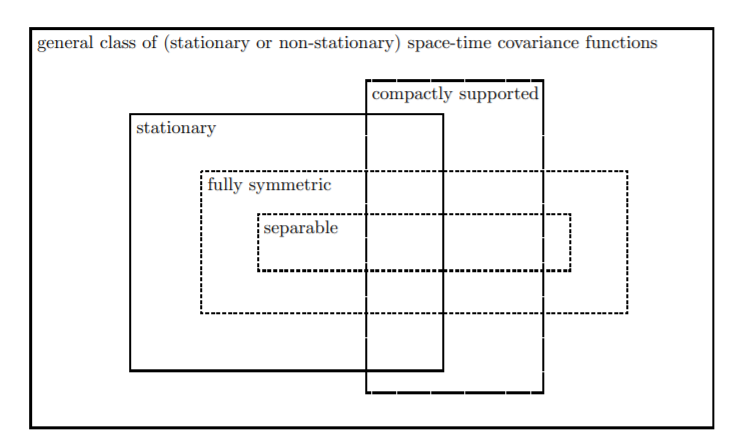
\includegraphics[width=10cm]{Gneiting.png}
    \caption{Relations: from technical note of Gneiting et al., \\ https://www.stat.washington.edu/sites/default/files/files/reports/2005/tr475.pdf}
\end{figure}
\begin{figure}[h]
    \centering
    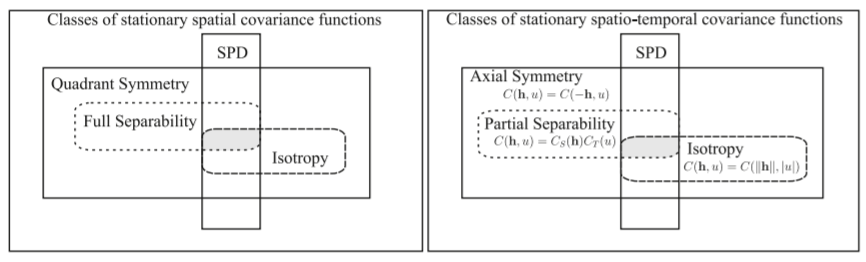
\includegraphics[width=16cm]{de_Laco.png}
    \caption{Relations: from S.De laco et al., 2019}
\end{figure}

\section{Reference}

Books:
\begin{itemize}
    \item Bochner, S. (1955). Harmonic analysis and the theory of probability. Courier Corporation.
    \item Matern, B. (1986). Spatial variation (Vol. 36). Springer Science \& Business Media.
    \item Stein, E. M., \& Shakarchi, R. (2003). Fourier analysis: an introduction (Vol. 1). Princeton University Press.
    \item Stein, E. M., \& Shakarchi, R. (2005). Real analysis: measure theory, integration, and Hilbert spaces. Princeton University Press.
    \item Stein, E. M., \& Shakarchi, R. (2011). Functional analysis: introduction to further topics in analysis (Vol. 4). Princeton University Press.
\end{itemize}

Papers:
\begin{itemize}
    \item Cressie, N., \& Huang, H. C. (1999). Classes of nonseparable, spatio-temporal stationary covariance functions. Journal of the American Statistical Association, 94(448), 1330-1339.
    \item Gneiting, T. (2002). Nonseparable, stationary covariance functions for space–time data. Journal of the American Statistical Association, 97(458), 590-600.
    \item Stein, M. L. (2005). Space–time covariance functions. Journal of the American Statistical Association, 100(469), 310-321.
    \item Porcu, E., Gregori, P., \& Mateu, J. (2006). Nonseparable stationary anisotropic space–time covariance functions. Stochastic Environmental Research and Risk Assessment, 21(2), 113-122.
    \item Porcu, E., Mateu, J., \& Saura, F. (2008). New classes of covariance and spectral density functions for spatio-temporal modelling. Stochastic Environmental Research and Risk Assessment, 22(1), 65-79.
    \item Porcu, E., Bevilacqua, M., \& Genton, M. G. (2016). Spatio-temporal covariance and cross-covariance functions of the great circle distance on a sphere. Journal of the American Statistical Association, 111(514), 888-898.
    \item De Iaco, S., Posa, D., Cappello, C., \& Maggio, S. (2019). Isotropy, symmetry, separability and strict positive definiteness for covariance functions: A critical review. Spatial statistics, 29, 89-108.
\end{itemize}
\end{document}